Una vez elegidos los valores representativos para la generación de lotes de secuencias, se realizaron 3 lotes Random de listas de secuencias (véase \texttt{secu\_20\_200\_10.in}, \texttt{secu\_20\_400\_20.in}, \texttt{secu\_20\_800\_40.in}) y se calcularon los tiempos de ejecución del algoritmo, obteniendo los resultados en los respectivos .out y las tablas de tiempos en los .times, con las que se obtuvieron los siguientes gráficos.
Estos archivos .in,.out y .times pueden verse en ej1/graficos\_y\_resultados/ .
\newline
\newline
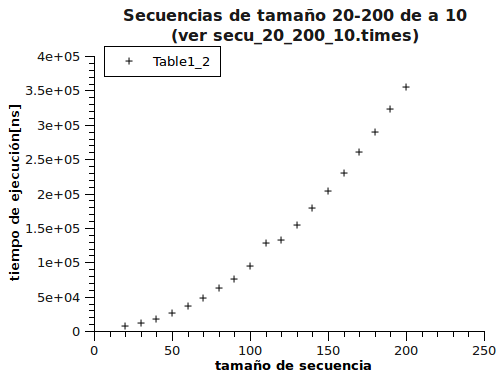
\includegraphics[scale=0.8]{img/ej1/Lote1.png}
\newline
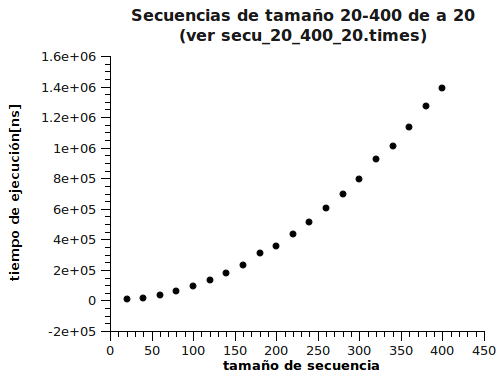
\includegraphics[scale=0.8]{img/ej1/Lote2.png}
\newline
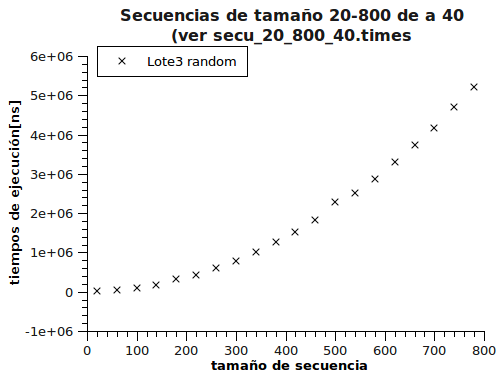
\includegraphics[scale=0.8]{img/ej1/Lote3.png}
\newline
